%---------- Inleiding ---------------------------------------------------------

\section{Introductie}%
\label{sec:introductie}

Voor het inlezen van MiFare kaarten worden card readers gebruikt, deze worden vaak verbonden met een web app die op de computer zelf draait. In deze bachelorproef gaat echter onderzoek worden gedaan naar een driver/extensie die het mogelijk maakt om de card reader te verbinden met een web app die online draait. Zo kunnen bijvoorbeeld toegangspassen worden ingelezen, dit is handig om te weten wie er zich in het gebouw bevindt voor moest het gebouw geëvacueerd worden bijvoorbeeld.

%---------- Stand van zaken ---------------------------------------------------

\section{State-of-the-art}%9
\label{sec:state-of-the-art}

\subsection{Wat is een browser extensie}
Op \textcite{Desktop.com} is te lezen dat een browser extensie een klein software programmatje is dat kan gebruikt worden om je web browser aan te passen en te verbeteren. Een extensie kan bestaande functies van de browser aanpassen, nieuwe toevoegen of aanpassen hoe de browser eruit ziet.
Een extensie kan bijvoorbeeld worden gebruikt om advertenties te blokkeren of om video's te downloaden van het internet.

\subsection{Wat is een driver}
Volgens \textcite{Webopedia} zorgen drivers voor de verbinding tussen een operating system en een hardware device of software applicatie. Zonder de drivers zou de hardware en software niet (goed) werken. Drivers vertellen aan de hardware of applicatie hoe ze moeten functioneren, dit gebeurt aan de hand van requests. Enkele apparaten die gebruik maken van driver zijn: Printers, Controllers, Modems en \textbf{Card readers}.

\subsection{Wat is een MiFare kaart}
Volgens \textcite{Digitalid} zijn MiFare kaarten contactloze kaarten die vroeger vooral populair waren als transport passen, maar tegenwoordig hebben ze hun populariteit vooral te danken aan het feit dat er data kan op worden bewaard dankzij de technologische mogelijkheden van de kaart.
De MiFare kaarten hebben net als andere contactloze kaarten een chip die wanneer ze in het magnetisch veld van een card reader komen erop gaan reageren. Ook maken ze gebruik van de ISO14443A industry-standard en werken ze op een frequentie van 13.56MHz.

\subsection{Voordelen van MiFare kaart}
Een MiFare kaart heeft volgens \textcite{Printplast} ook enkele voordelen. Het eerste voordeel is dat de kaart kan ingelezen worden van een maximum afstand van 10cm wat de gebruiker een touch-and-go beleving geeft.
Het maakt ook gebruik van een beveiligingsencryptie dat moeilijk te clonen is. Ook supporten MiFare kaarten een multi interface, dit wil zeggen dat het buiten contactloos inlezen ook mogelijk is om de kaart met contact in te lezen. En tenslotte kan de technologie buiten kaarten ook gebruikt worden in bijvoorbeeld sleutelhangers en smartphones.

\subsection{Waarvoor worden MiFare kaarten gebruikt}
Door de vele voordelen van een MiFare kaart kan deze volgens \textcite{Digitalid} voor veel dingen worden gebruikt, hier zijn enkele voorbeelden: Campus/studentenkaarten, transport tickets, event tickets, bib kaarten, hotelsleutelkaarten en bankkaarten.

\subsection{Wat zijn Web NFC en Web USB}
Volgens een artikel van \textcite{FrançoisBeaufortUSB} zorgt Web USB ervoor dat USB apparaat services kunnen worden gebruikt op het Web. Met deze API hebben hardware fabrikanten de mogelijkheid om cross-platform SDK’s te bouwen voor hun apparaten. Maar het belangrijkste voordeel is dat het USB veiliger maakt door het naar het Web te brengen.
NFC staat voor ‘Near Field Communication’, de communicatie tussen het scan toestel en de tag gebeurt volgens \textcite{FrançoisBeaufortNFC} op een afstand van minder dan 10 centimeter. Web NFC zorgt ervoor dat je via sites read en write acties kan uitvoeren op een NFC tag die zich in de buurt van het scan toestel bevindt. Web NFC maakt gebruik van het NFC Data Exchange Format (NDEF) om data uit te wisselen, dit omdat de security eigenschappen van NDEF makkelijker kwantificeerbaar zijn.
Over het algemeen geldt dat als de kaartlezer een USB-interface gebruikt en nauwkeurige controle over de communicatie met het apparaat nodig is, Web USB waarschijnlijk de betere optie is. Als de kaartlezer NFC gebruikt en een hoogwaardige API nodig is voor het lezen en schrijven van NFC-tags, is Web NFC wellicht de betere optie.

\subsection{Stappen om de driver te maken}
Om de driver te maken die ervoor moet zorgen dat de kaartlezer met de browser kan worden verbonden kunnen over het algemeen de volgende stappen worden gevolgd:
\begin{itemize}
    \item 1. Bepaal de communicatie-interface van de kaartlezer (bijv. USB, seriële poort, Bluetooth).
    \item 2. Schrijf de code voor de communicatie tussen de kaartlezer en de computer via de interface.
    \item 3. Implementeer de code voor de communicatie-interface als onderdeel van het besturingssysteem van de computer.
    \item 4. Schrijf de code om de kaartlezer te detecteren en een bericht te sturen naar de webbrowser.
    \item 5. Implementeer de code in de webbrowser om de kaartlezer te detecteren en met de juiste toestemming toegang te krijgen tot de kaartinformatie.
\end{itemize}

\subsection{Server-Sent Events}
Server-sent Evens zorgen volgens \textcite{DigitalOceanSSE} voor real-time updates van data in een webapplicatie. Aan de client kant voorziet het hiervoor de EventSource API, met behulp van deze API kan er geconnecteerd worden met de server en updates ontvangen. Dus als de server een update verstuurt dan gaat de client side, die dus eigenlijk geabonneerd is op de server, deze data van de server meteen ontvangen en kan de website direct worden geüpdate.

\subsection{Windows Services}
Windows services zijn volgens \textcite{MicrosoftWS} applicaties die voor lange tijd runnen. Ze kunnen automatisch worden opgestart wanneer de computer wordt gestart en maken geen gebruik van een interface. Services draaien dus vaak op de achtergrond zonder dat de gebruiker er iets van merkt. Via de Windows Service Manager kunnen services worden beheert. Een service zou in dit geval goed van pas kunnen komen om de MiFare kaart uit te lezen en de data ervan door te sturen. Door de kaart op de card reader te leggen zal de service de data van die kaart behandelen voor de gebruiker.

%---------- Methodologie ------------------------------------------------------
\section{Methodologie}%
\label{sec:methodologie}

In de eerste fase van het onderzoek zal er een literatuurstudie worden gedaan over het maken van een driver, MiFare- en smartcards en de card reader. Uit de state-of-the-art bleek al dat WebUSB een potentiële oplossing is. Om verdere oplossingen te vinden zal er in het tweede fase van de bachelorproef een interview worden afgelegd bij de co-promotor, omdat hij een idee heeft voor een andere mogelijke oplossing. Dit idee omvat Windows Services en Server-sent events. Vervolgens zullen deze potentiële oplossingen (indien mogelijk) worden uitgewerkt tot een Proof of Concept. En tenslotte zal er een vergelijkende studie worden gedaan op basis van de Proof of Concepts om te kijken welke mogelijke oplossing het beste is. De uiteindelijke PoC zal Jan De Nul dan kunnen gebruiken om MiFare cards in te lezen op hun webapplicatie. 

\begin{center}
    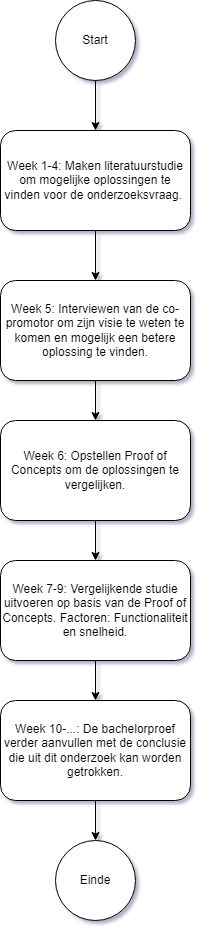
\includegraphics[width=4cm]{flowChart3}
\end{center}

%---------- Verwachte resultaten ----------------------------------------------
\section{Verwacht resultaat}%
\label{sec:verwachte_resultaten}

Het verwachte resultaat zal een werkende extensie/driver zijn die ervoor zorgt dat een webapplicatie MiFare kaarten rechtstreeks in kan lezen in de browser. Via die webapplicatie zal men de mogelijkheid hebben om toeganskaarten en maaltijdcheques in te scannen om zo het start/stop uur in te geven of gebruik te kunnen maken van de cheques door de persoon die gelinkt is aan de kaart.

\section{Verwachte conclusies}%
\label{sec:Verwachte_conclusies}

Uit deze bachelorproef moet duidelijk blijken dat het mogelijk is om een card reader rechtstreeks te verbinden met een web app vanuit de browser. De PoC zal aantonen dat dit mogelijk is en dat er dus MiFare kaarten ingescand kunnen worden in de web app waardoor die gebruik zal kunnen maken van data op de kaart om toegangskaarten of maaltijdcheques te kunnen beheren. Hopelijk vloeit uit dit onderzoek een PoC die klaar is voor de consument die opzoek is naar een extensie/driver voor het inlezen van chipkaarten in zijn webapplicatie.